\section{Simulation Analysis}
\label{sec:simulation analysis}
\subsection{Optimizer}
In order to maximize the M value, we started with a simple  circuit, and tried to make small changes and evaluate their results. The main changes were the value of the parameters of the chosen components, their number, and their location.

We realised that the manual optimization was going to be a long and difficult process, so we decided to create a simple optimizer to do it autonomously.

It has the capacity to change the capacitance of the Capacitor, the resistance of the resistor, the N value of the transformer, and the number of diodes. We found that it worked best if we fixed the values of some of these parameters. The combination that worked best for us was fixing the capacitor value, N value and the Diode Value, and only optimize the the transformer and capacitor.  That means that we still had to tinker with the number of diodes and the resistance, but it was much less work intensive than tinkering with all the variables.

The program works by doing small variations of the values and evaluating their effect. It starts with a starting configuration. Then it chooses a parameter to variate at random, and varies it a random amount. Then it checks if it is better than the current best one. The second variation is done to the best performer, the combination with the best M value. This means that the best M value keeps improving if the program finds a best combination at random.

We ended up leaving the program for a few minutes for short optimization sessions, and found that the program had a high tendency to get the average voltage on point with the 12v, as expected. It also ran much faster than we were expecting. It ended up being a win win situation in our eyes, and it can be found in our git repo. Note that upon executing the code, since the results are tied to random values, the final answer might not be exactly the same as ours. It might even be better if it is given enough time.


\begin{table}[h]
  \centering
  \begin{tabular}{|l|r|}
    \hline    
    %{\bf Name} & {\bf Value [A or V]} \\ \hline
    Component & Parameter Value \\
    \hline
    Resistor & 45 k\Omega \\
    \hline
    Capacitor & 17.5150173805745 \mu F \\
    \hline
    Number of diodes in the Voltage Regulator & 19 Diodes \\
    \hline
    Number of diodes in the full wave rectifier & 4 Diodes \\
    \hline
    N value of the transformer & 7.29150093083668 \\
    \hline
    Total cost & 64.81501 MU \\
    \hline
  \end{tabular}
  \caption{Table of costs. Note that the total cost is sum of the the other values (in this units, with the number of diodes multiplied by 0.1).}
  \label{tab:components}
\end{table}

\subsection{Spice Results}
 Using the values stated above and using them in a simulated circuit in ngspice as shown in the circuit shown in Figure \ref{fig:circuit} we obtain the following results.
 

\begin{table}[h]
  \centering
  \begin{tabular}{|l|r|}
    \hline    
    %{\bf Name} & {\bf Value [A or V]} \\ \hline
    \input{../sim/info}
  \end{tabular}
  \caption{Spice results. The M value and the cost were calculated by an additional octave script included in the git.}
  \label{tab:info}
\end{table}

\vspace{1cm} 
In the following image the blue line represents the voltage at the of the envelope detector, the red represents the voltage obtained by the transformer, and last, the orange represents the output voltage in the voltage detector.

\begin{figure}[!h]
    \centering
      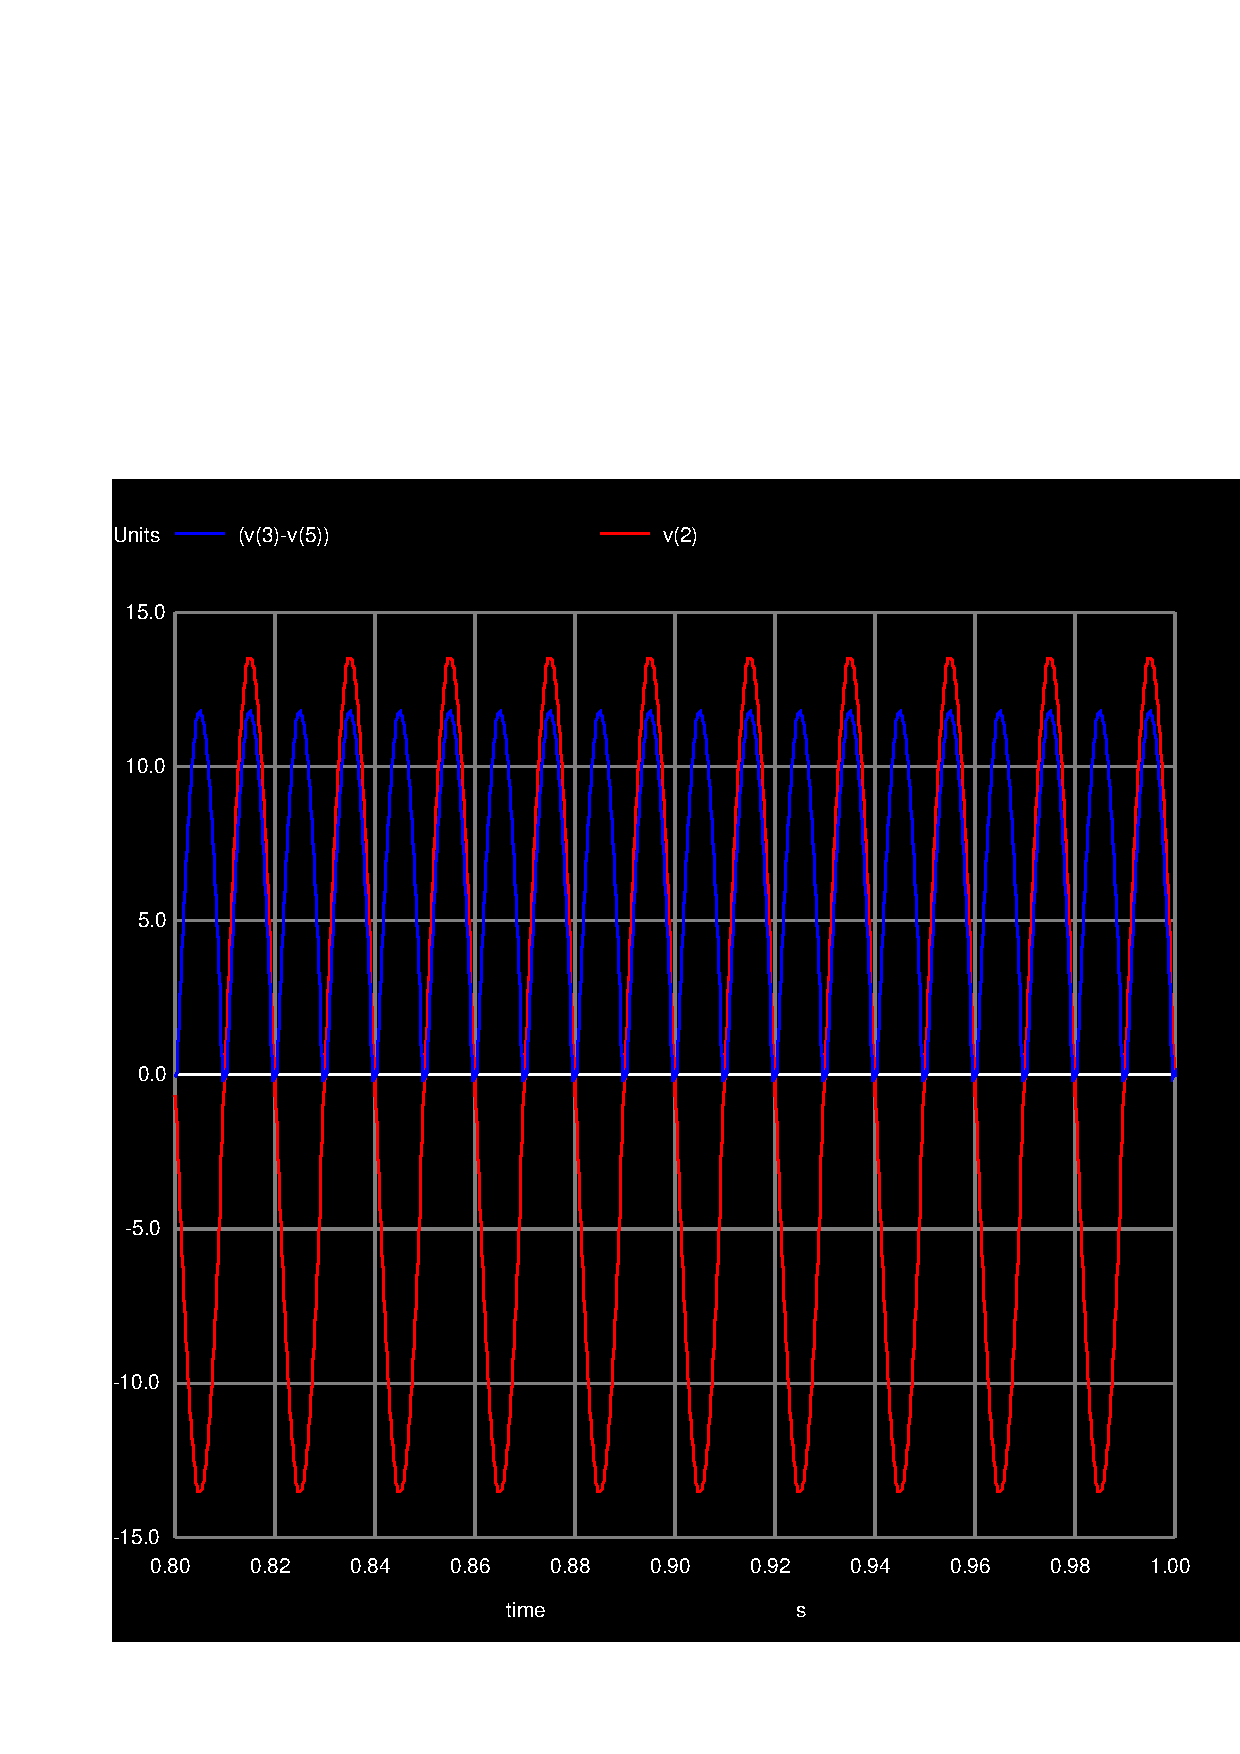
\includegraphics[width=.45\columnwidth]{../sim/outputvoltage.pdf}
      \caption{Detailed view}
      \label{fig:trans3}
\end{figure}


\begin{figure}[!h]
    \centering
      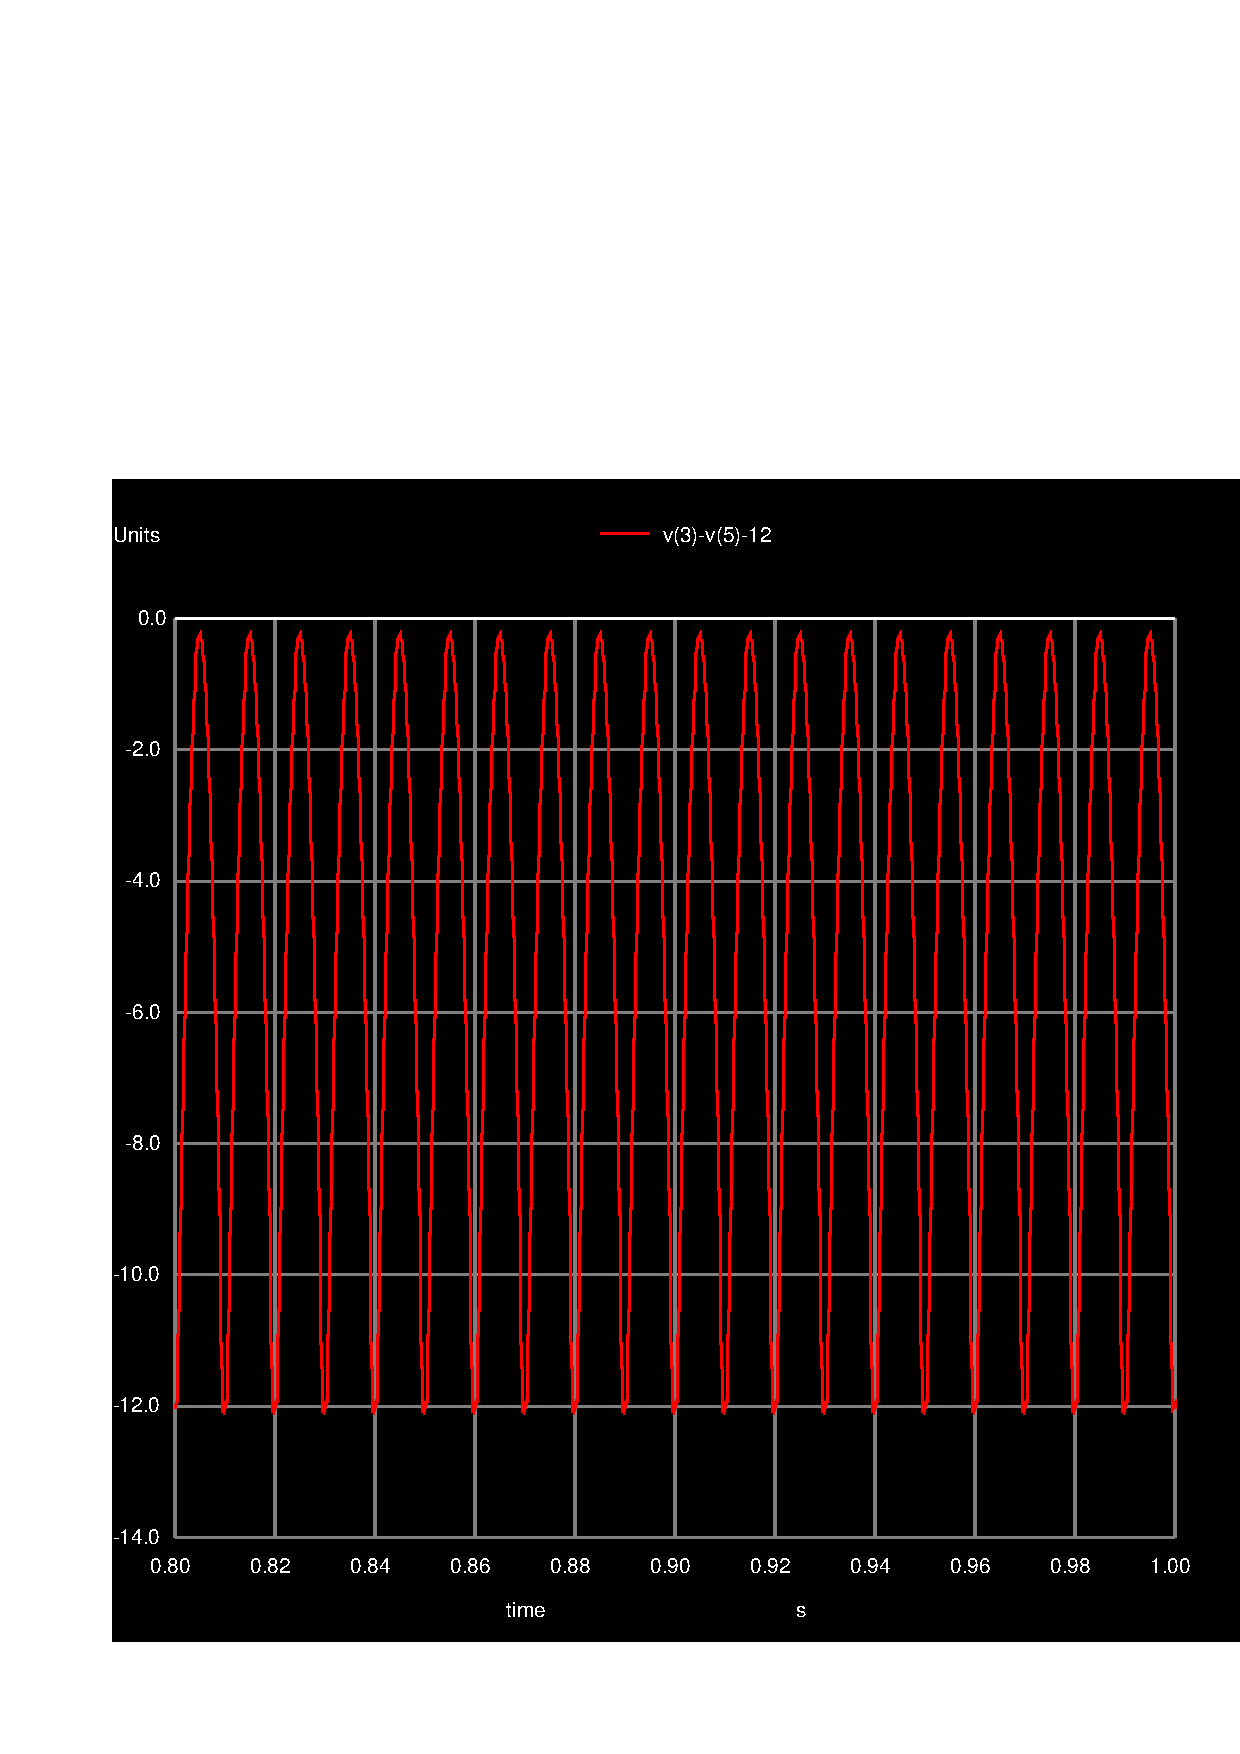
\includegraphics[width=.45\columnwidth]{../sim/detail.pdf}
      \caption{Detailed view}
      \label{fig:trans3}
\end{figure}

\subsection{Simulation values for the theoretical analysis}

In the Figure \ref{fig:Rd} we can see the results of small variations of the voltage values in the current that passes through the diodes (simulated using ngspice).

By definition, the incremental resistance in the diode can be calculated by $\frac{dv}{di} = \frac{1}{\frac{di}{dv}}$.

We then approximate the value of the derivative to its finite derivative, which is the value of the slope in \ref{fig:Rd}.

Lastly, to calculate the value of the incremental resistance of one diode, we divide the value obtained previously by the number of the diodes, leading to a final 65.7894736842105 $\Omega$.




\begin{figure}[!htb]
    \centering
      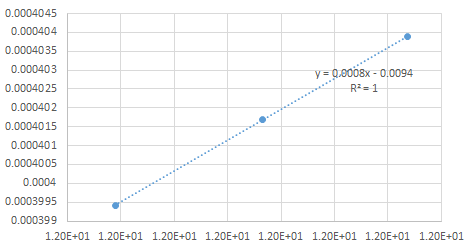
\includegraphics[width=.6\columnwidth]{Rd.png}
      \caption{Current (in A) in function of the voltage (in V)}
      \label{fig:Rd}
\end{figure}
